\documentclass[twoside,11pt]{article}
\pdfinfoomitdate=1
\pdftrailerid{termgraph}

\usepackage[preprint,nohyperref]{jmlr2e}
\usepackage{amsmath,amssymb}
\usepackage{booktabs}
\usepackage{graphicx}
\usepackage{float}

\graphicspath{{../assets/figures/}}
\renewcommand{\arraystretch}{1.18}
\setlength{\emergencystretch}{2em}

\ShortHeadings{TermGraph}{Mery Caro}
\firstpageno{1}

\title{TermGraph: A Certified Glassbox Exchange Architecture for GBM-Class Models}

\author{\name Patricio Alejandro Mery Caro \\
       \addr Independent Researcher, La Serena, Chile}

\begin{document}
\raggedbottom
\maketitle

\begin{abstract}
Gradient-boosted trees are still the default for tabular prediction. Their
explanations are post hoc, and the deployed artifact cannot be edited.
Explainable boosting machines (EBMs) and neural additive models (NAMs) are
glassboxes, but both are fixed-order learners; neither acts as an exchange layer
for an existing GBM. TermGraph compiles a GBM into a sum of low-order table
terms. The term ledger is exact, feature values use a declared sharing
convention, terms can be edited after training, and a controller chooses between
compact and max-accuracy artifacts. On the KIRK planetary-stability task, a
22-term TermGraph compiled from an EBM plus an order-3 residual reaches
$0.9427 \pm 0.0048$ AUC over five seeds, against $0.9417 \pm 0.0049$ for EBM
GA$^2$M and $0.9206$ for NAM. A five-term compact artifact reaches $0.9296$ at
the same budget, where EBM reaches $0.9252$. On a controlled 3-way
benchmark, TermGraph reaches $0.8297$ against $0.6989$ for pairwise EBM. The
certified 22-term table matches its source to
$5.3\times10^{-15}$ maximum logit error, and a fused runtime reaches $8.72\times$
on eight threads ($5.66$M rows/s) with a $0.66$~MB binary artifact. I also
report where EBM remains the better choice and where a marginal ANOVA
diagnostic gives a misleading picture.
\end{abstract}

\begin{keywords}
glassbox models, explainable artificial intelligence, explainable boosting machines, SHAP, gradient boosting, tabular data
\end{keywords}

\section{Introduction}

Tabular prediction is still dominated by gradient-boosted decision trees
(GBMs) such as XGBoost, LightGBM, and CatBoost~\citep{chen2016xgboost,ke2017lightgbm,prokhorenkova2018catboost}.
They are accurate and robust, and they are easy to tune. The deployed object,
however, is an ensemble of trees whose decisions cannot be inspected directly.
SHAP and TreeSHAP~\citep{lundberg2017shap,lundberg2020tree} give post-hoc
attributions, but the explanation remains a separate object: it cannot be
edited, it depends on a baseline, and it does not give a replacement model.

Additive glassboxes take a different route. Generalized additive models
(GAMs)~\citep{hastie1990gam}, explainable boosting machines
(EBMs/GA$^2$M)~\citep{lou2012intelligible,lou2013accurate}, and neural additive
models (NAMs)~\citep{agarwal2021nam} describe the prediction as a sum of
low-order functions. This makes the model readable, but the hypothesis class is
fixed in advance. EBM stops at pairwise interactions; NAM stops at univariate
shapes. Neither can take an existing GBM and return a certified, editable
artifact.

I ask whether a glassbox can serve as that exchange layer. I test the question
on KIRK, a planetary-stability classifier, and on a matched synthetic benchmark.
Both tests support the role. A 22-term TermGraph matches the EBM plus order-3
hybrid, and a five-term artifact is competitive at the same term budget. EBM
remains the better low-order model, which is a useful boundary rather than a
defect.

A term graph represents the model as a sum of low-order tables. A compiler turns
EBM terms and a constrained XGBoost term into those tables, and a Glassbox
Contract plus a budget controller decide which artifact can be deployed. The
empirical section reports the KIRK comparison, a controlled 3-way test, post-hoc
term edits, and the runtime. I keep the negative results in the paper because
they mark where the claim stops.

\section{Related Work}

Research on additive glassboxes begins with GAMs~\citep{hastie1990gam}, which
model a response as a sum of univariate shape functions. EBM and
GA$^2$M~\citep{lou2012intelligible,lou2013accurate} add pairwise terms with
boosted stumps; InterpretML provides a practical
implementation~\citep{nori2019interpretml}. NAM~\citep{agarwal2021nam} replaces the
shape functions with small neural networks. These are the closest baselines, and
they are the reason the paper reports where TermGraph wins instead of making a
blanket claim.

Post-hoc attribution follows a different tradition. SHAP~\citep{lundberg2017shap}
is the standard attribution framework, and TreeSHAP~\citep{lundberg2020tree} is
exact for tree ensembles. The limitation is structural: a post-hoc explanation
is not a model artifact and cannot be edited. Rudin~\citep{rudin2019stop} argues
for inherently interpretable models when stakes are high. TermGraph follows that
direction and adds an exchange and certificate layer.

XGBoost, LightGBM, and CatBoost~\citep{chen2016xgboost,ke2017lightgbm,prokhorenkova2018catboost}
define the accuracy envelope for tabular learners. TermGraph uses XGBoost for
the order-3 term and EBM for the low-order terms. The deployed object is a
table graph, not a tree ensemble.

\section{Architecture}

\subsection{Term graph and blocks}

A TermGraph is
\begin{equation}
  f(x) = b + \sum_{j=1}^{K} g_j(x_{S_j}), \qquad |S_j| \le d,
  \label{eq:model}
\end{equation}
where $S_j \subseteq [p]$ is the support of term $j$, $g_j:\mathbb{R}^{|S_j|}\to\mathbb{R}$
is a centered term, and $b$ is the bias. Supports may overlap; the graph is a
hypergraph. Complexity is the vector
\begin{equation}
  C(G) = (K,\, d,\, \text{overlap},\, \text{cells}),
  \qquad
  \text{overlap} = \max_i |\{j:i\in S_j\}|.
\end{equation}
The implementation exposes a reusable block specification
(\texttt{TermBlock}: inputs, basis, learner, composition, order) and a
\texttt{ModelSpec} for candidate artifacts. The compact artifact is a partition
of the 11 features; the max-accuracy artifact is a declared hypergraph.

\begin{figure}[t]
  \centering
  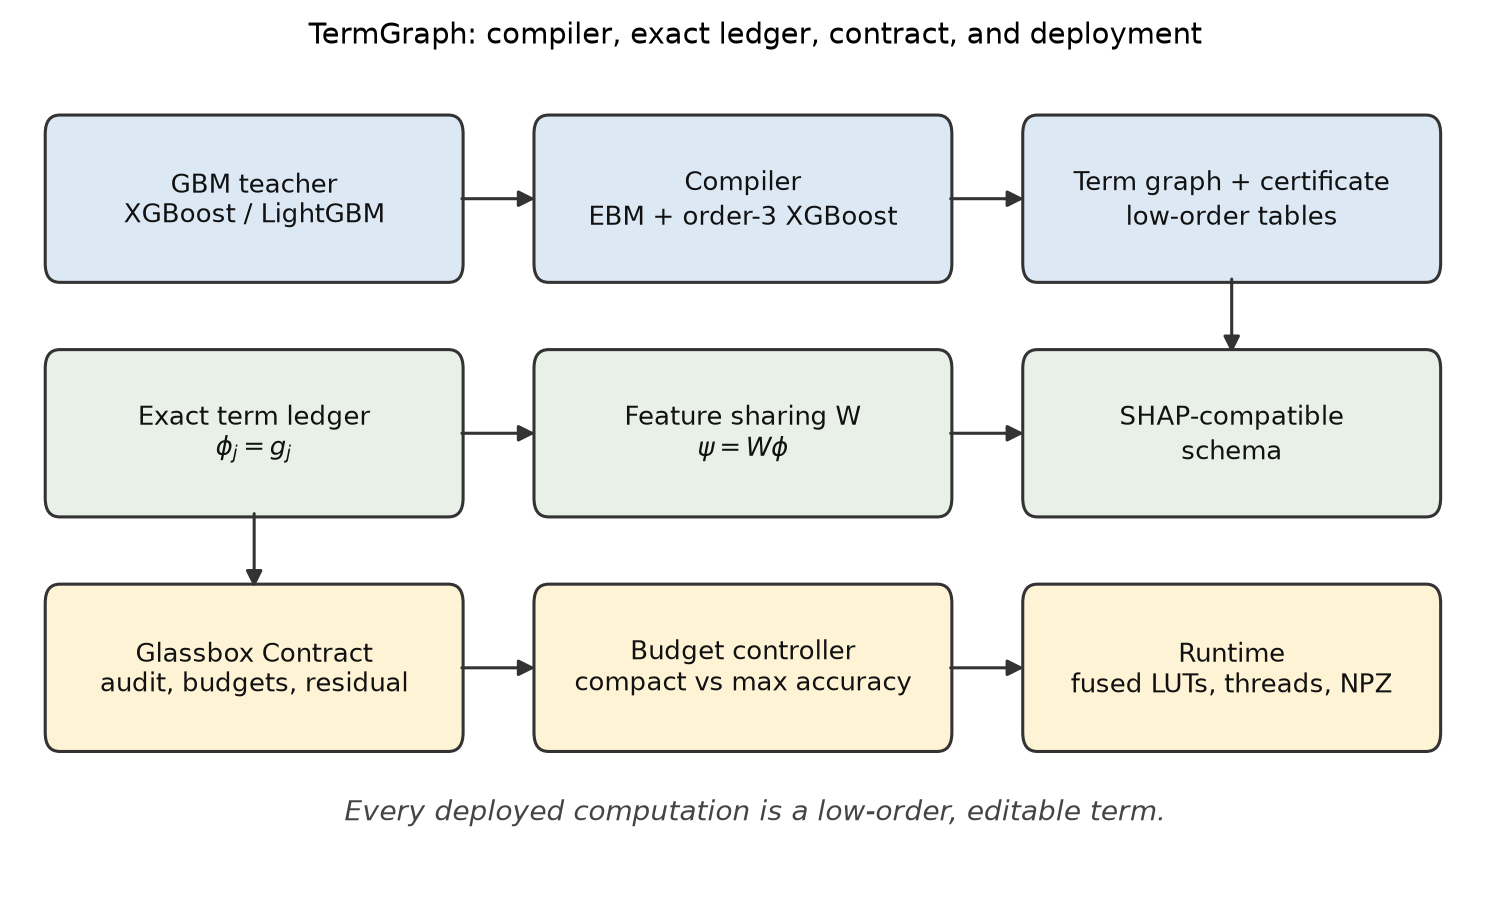
\includegraphics[width=\linewidth]{fig_architecture}
  \caption{TermGraph compiles a GBM into a low-order term graph. The exact term
  ledger, declared feature sharing, Glassbox Contract, controller, and fused
  deployment runtime are separate layers.}
  \label{fig:architecture}
\end{figure}

\subsection{Glassbox Contract}

A deployed graph is admissible only if
\begin{equation}
  K \le K_{\max},\quad d \le d_{\max},\quad \text{cells} \le C_{\max},\quad
  \text{additivity} \le \varepsilon,\quad \text{certificate present}.
\end{equation}
The contract also requires a rendering protocol: a 1D curve, a 2D heatmap, or
3D slices. Cell count alone is not readability. The controller refuses a budget
that no admissible artifact can meet.

\section{Mathematical Core}

\subsection{Table terms}

For term $j$ and input $l$, let $e_{j,l,0}<\cdots<e_{j,l,m_{j,l}}$ be explicit
edges, with sentinel outer edges. The bin index is
\begin{equation}
  \kappa_{j,l}(x_l) = \operatorname{clip}\big(
  \operatorname{searchsorted}(e_{j,l},x_l)-1,\;0,\;m_{j,l}-1\big),
\end{equation}
and the term is
\begin{equation}
  g_j(x_{S_j}) = \theta_j[\kappa_{j,1}(x_{i_1}),\ldots,
  \kappa_{j,|S_j|}(x_{i_{|S_j|}})] - c_j,
\end{equation}
where $\theta_j$ is the value table and $c_j$ is the centering constant. A table
compiler is exact iff the source term is constant on every cell of the Cartesian
product of its edges.

\subsection{Two attribution levels}

The \emph{term ledger} is
\begin{equation}
  \phi_j(x) = g_j(x_{S_j}), \qquad f(x)=b+\sum_j \phi_j(x),
\end{equation}
which is exact by construction. Feature attribution uses a sharing matrix
$W\in\mathbb{R}^{p\times K}$:
\begin{equation}
  W_{i,j}\ge 0,\quad W_{i,j}=0\ \text{if }i\notin S_j,\quad
  \sum_i W_{i,j}=1,\quad
  \psi_i(x)=\sum_j W_{i,j}\phi_j(x).
\end{equation}
The default is equal split, $W_{i,j}=1/|S_j|$. This is the Shapley value of the
within-term symmetric game, \emph{not} the full-model Shapley value when terms
overlap. If full-model Shapley is required, it must be computed separately; the
ledger is a coarsening.

\subsection{Two order definitions}

Under a product baseline $P_\perp$, the functional-ANOVA tail energy is
\begin{equation}
  E_{>d}=\sum_{|A|>d}\operatorname{Var}_{P_\perp}(f_A).
\end{equation}
This bounds approximation under $P_\perp$, not under the data distribution $P$.
The effective order is
\begin{equation}
  d_{\mathrm{eff}}(P,\delta)=\min\{d:R_d(P)-R^*(P)\le \delta\}.
\end{equation}
The two can disagree sharply: on KIRK, marginal ANOVA assigns only $43.3\%$ of
the energy to order $\le3$, while an order-3 glassbox captures $93.5\%$ in
distribution. The paper reports both and does not use the marginal number as the
deployment limit.

\subsection{Exactness}

Table~\ref{tab:exactness} separates the exact claims from the conventions. The
term ledger is exact by construction; feature values use a declared sharing
matrix; the marginal ANOVA tail is a product-baseline diagnostic, not a
data-distribution guarantee.

\begin{table}[t]
\centering
\normalsize
\setlength{\tabcolsep}{4pt}
\begin{tabular}{@{}lll@{}}
\toprule
Claim & Exact? & Caveat \\
\midrule
$f=b+\sum_j\phi_j$ & yes & by construction \\
table compiler & yes iff constant on cells & otherwise $\delta$ \\
term ledger $\phi_j$ & yes & baseline $P$ declared \\
feature attribution $\psi_i$ & convention & sharing matrix $W$ \\
full-model Shapley & separate computation & not the ledger when overlapping \\
marginal ANOVA tail $E_{>d}$ & yes under $P_\perp$ & not the $P$ limit \\
\bottomrule
\end{tabular}
\caption{Exactness claims in this paper, separated by object. The term ledger is
exact by construction. Feature attribution is a declared sharing convention, not
full-model Shapley. The marginal ANOVA tail is a product-baseline diagnostic and
does not bound the data-distribution risk.}
\label{tab:exactness}
\end{table}

\section{KIRK Case Study}

\subsection{Data and protocol}

KIRK classifies the long-term stability of compact planetary systems from a
short integration~\citep{tamayo2020spock,thadhani2025spock,hussain2020shadows,rein2017rebound}.
The cache contains 12,000 real initial conditions with 11 SPOCK 2.0 features;
9,767 are short-stable and used for training and evaluation. The teacher is the
SPOCK 2.0 XGBoost classifier~\citep{thadhani2025spock}. The target is the real
$10^9$-orbit label. I use five seeds, an 85/15 split, and exclude short-unstable
systems from scoring, following the KIRK protocol.

The max-accuracy artifact uses an EBM GA$^2$M with 10 pairwise interactions for
the low-order terms and one constrained XGBoost order-3 residual term on
\texttt{EMcrossnear}, \texttt{MMRstrengthnear}, and \texttt{EMfracstdnear}. The
compact artifact uses a partition of five terms: one 3-way block and four pairs.

\subsection{Baselines and metrics}

Baselines are NAM, EBM GAM, EBM GA$^2$M, an unconstrained XGBoost student trained
on the same data, and the SPOCK teacher. The primary metric is AUC against the
real labels; I also report log-loss and accuracy.

\begin{table}[t]
\centering
\normalsize
\setlength{\tabcolsep}{3.5pt}
\begin{tabular}{@{}lcccc@{}}
\toprule
Model & Terms & AUC truth & Log-loss & Accuracy \\
\midrule
NAM 12k & 11 & $0.9206\pm0.0068$ & -- & 0.8409 \\
EBM GAM & 11 & $0.9386\pm0.0054$ & 0.2992 & -- \\
EBM GA$^2$M & 21 & $0.9417\pm0.0049$ & 0.2917 & 0.8718 \\
TermGraph max (EBM + order 3) & 22 & $\mathbf{0.9427\pm0.0048}$ & \textbf{0.2895} & \textbf{0.8729} \\
TermGraph compact & 5 & 0.9296 & 0.3200 & 0.8615 \\
EBM at 5-term budget & 5 & 0.9252 & -- & -- \\
Unconstrained XGBoost & -- & 0.9381 & -- & -- \\
SPOCK teacher & -- & 0.9566 & -- & -- \\
\bottomrule
\end{tabular}
\caption{KIRK results. AUC is against the real $10^9$-orbit labels and higher is
better; log-loss is lower. The max and EBM GA$^2$M rows are five-seed means. The compact row is
the deployed five-term artifact on its certified fold. EBM at the five-term
budget uses five features because EBM needs one term per feature. The
unconstrained XGBoost row is the clean internal-validation reference, and the
teacher is the 100k SPOCK model.}
\label{tab:kirk}
\end{table}

\subsection{Results}

Table~\ref{tab:kirk} reports the KIRK comparison; the max and EBM GA$^2$M
rows are five-seed means. The max model reaches $0.9427\pm0.0048$ AUC over five
seeds, against $0.9417\pm0.0049$ for EBM GA$^2$M and $0.9206$ for NAM. The
paired gain over EBM is $+0.0010$, and it is positive on all five seeds. The
compact artifact reaches $0.9296$ at a five-term budget, while EBM reaches
$0.9252$ because it cannot merge features into multi-feature terms.

Figure~\ref{fig:kirk} shows the paired seeds and the fixed-budget comparison.
The comparison is mixed. On raw KIRK AUC, EBM GA$^2$M ($0.9417$) beats both the
deployed compact artifact ($0.9296$) and the earlier full-capacity five-term
experiment ($0.9364$). The defensible claim is narrower. TermGraph adds order 3
and keeps a certified, editable ledger, and it does so without losing the
low-order baseline.

\begin{figure}[t]
  \centering
  \begin{minipage}[t]{0.48\linewidth}
    \centering
    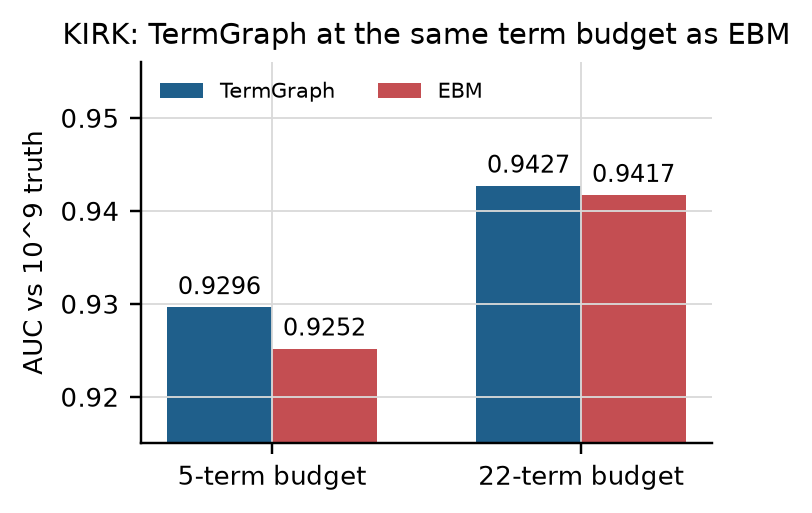
\includegraphics[width=\linewidth]{fig_budget}
    \par\smallskip
    {\small (a) AUC at five and 22 terms. The five-term TermGraph uses all 11
    features; the five-term EBM uses five.}
  \end{minipage}\hfill
  \begin{minipage}[t]{0.48\linewidth}
    \centering
    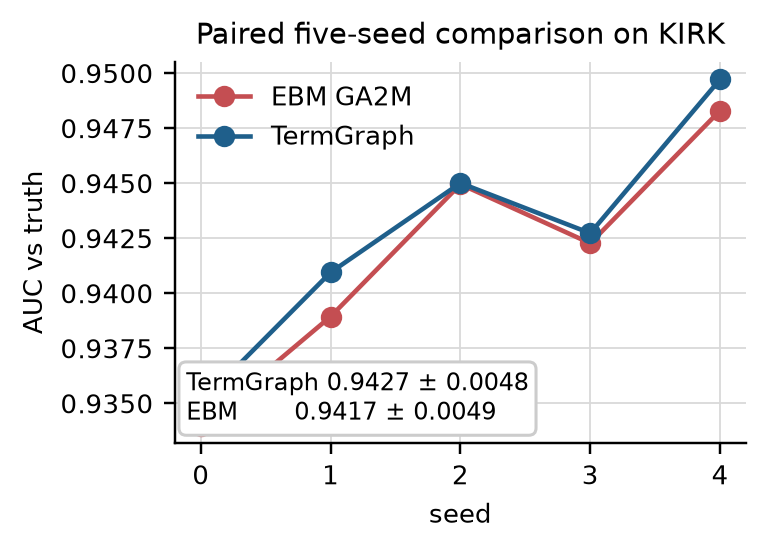
\includegraphics[width=\linewidth]{fig_five_seed}
    \par\smallskip
    {\small (b) Paired seeds. Each line is one 85/15 split; both models use the
    same split.}
  \end{minipage}
  \caption{KIRK performance. The compact artifact is competitive at a five-term
  budget, and the max artifact matches the EBM plus order-3 hybrid on the same
  five seeds.}
  \label{fig:kirk}
\end{figure}

\subsection{Compilation and hardware}

Figure~\ref{fig:hardware} reports the deployment and edit measurements. The
EBM terms are compiled with EBM's own cut points; the 3-way term uses the
union of its tree thresholds. On the certified fold, the table matches the
EBM + order-3 hybrid to $5.3\times10^{-15}$ maximum logit error, and additivity
is $0.0$. A fused runtime bins each unique feature/edge pair once per batch,
flattens term tables, and accumulates without materializing the $(n,K)$ matrix.
On 200,000 rows it reaches $8.72\times$ on eight threads ($5.66$M rows/s) with a
maximum difference of $5.3\times10^{-15}$. The binary NPZ artifact is $0.66$~MB
versus $6.0$~MB JSON and loads $7.4\times$ faster.

\begin{figure}[H]
  \centering
  \begin{minipage}[t]{0.48\linewidth}
    \centering
    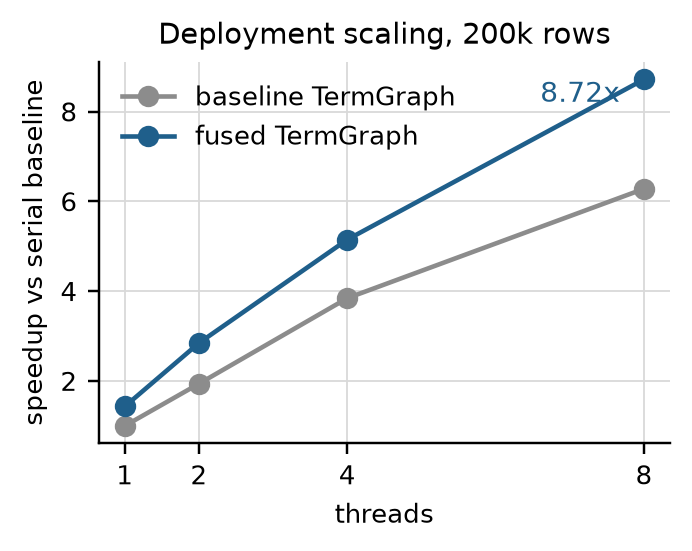
\includegraphics[width=\linewidth]{fig_parallel}
    \par\smallskip
    {\small (a) Speedup against the serial baseline on 200k rows. The fused
    runtime bins each unique feature and edge set once per batch.}
  \end{minipage}\hfill
  \begin{minipage}[t]{0.48\linewidth}
    \centering
    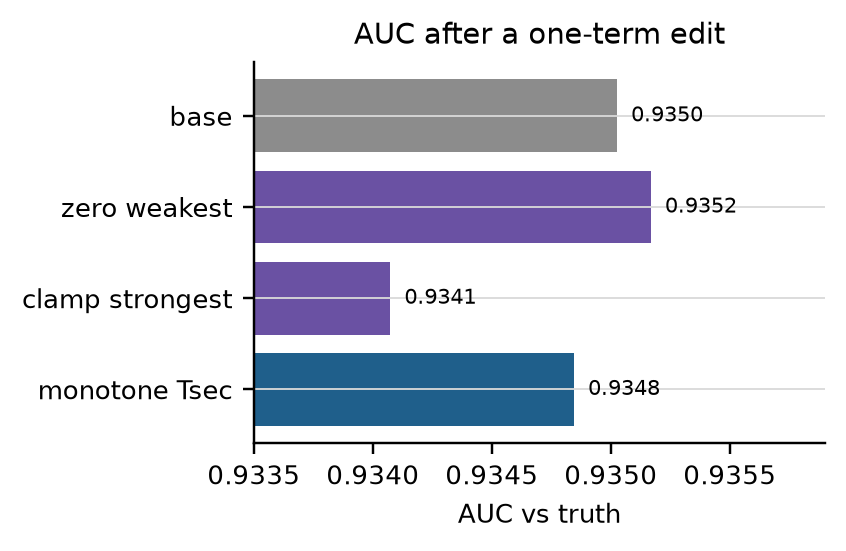
\includegraphics[width=\linewidth]{fig_edit}
    \par\smallskip
    {\small (b) AUC before and after zeroing, clamping, or monotonizing one term.
    The remaining-term maximum delta is 0.0.}
  \end{minipage}
  \caption{Fused table inference and post-hoc term surgery. The edits change one
  term and leave the other term contributions unchanged; log-loss improves for
  the clamp and monotone edits.}
  \label{fig:hardware}
\end{figure}

\subsection{Term surgery and the controller}

Zeroing the weakest term changes only that term; the remaining-term maximum
delta is $0.0$. Clamping the strongest term and enforcing monotonicity in
\texttt{Tsec} also leave the rest unchanged; the monotone edit reduces 1,365
violations to zero while improving log-loss. The controller selects the compact
artifact at budgets 5--6 and the max artifact at 22; budget 4 returns no
admissible model.

\subsection{Data scaling}

Figure~\ref{fig:scaling} reports the scaling record. It cautions against reading
the five-seed result as a 100k-data claim. From 1k to 8.3k truth-labelled
systems, TermGraph improves from $0.9152$ to $0.9349$ AUC; distillation of the
teacher plateaus around $0.9264$; the unconstrained GBM improves from $0.9104$ to
$0.9384$. Truth labels scale, distillation saturates, and the full 100k archive
was not trained here.

\begin{figure}[t]
  \centering
  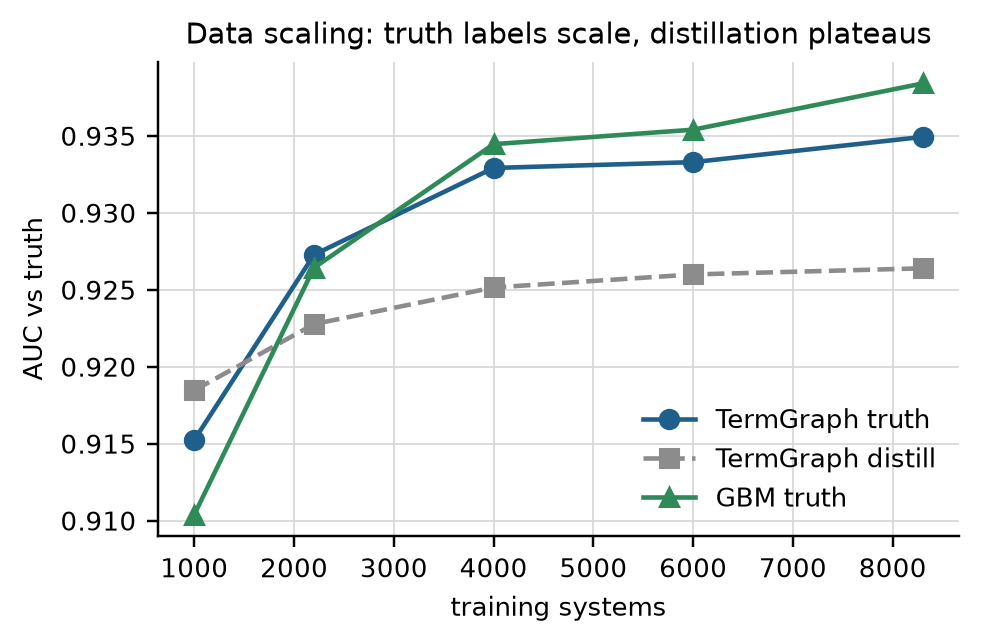
\includegraphics[width=0.62\linewidth]{fig_scaling}
  \caption{Data scaling. The x-axis is the number of truth-labelled training
  systems, and the y-axis is AUC against truth. Truth-label training keeps
  improving; teacher distillation plateaus. The full 100k archive is out of
  scope.}
  \label{fig:scaling}
\end{figure}

\section{Controlled 3-way Test}

Figure~\ref{fig:synthetic} reports the controlled test. I generate three synthetic truths: additive,
pairwise, and 3-way (within-block 3-way terms, no cross-block pairs). The
matched TermGraph uses the corresponding blocks; EBM uses 10 pairwise
interactions; the unconstrained GBM is the reference.

On the 3-way truth, TermGraph reaches $0.8297\pm0.0034$ AUC, the unconstrained
GBM $0.8217\pm0.0018$, and EBM GA$^2$M $0.6989\pm0.0022$. On the pairwise truth,
TermGraph and EBM are statistically comparable ($0.8304$ vs $0.8319$), and both
beat the unconstrained GBM ($0.8255$). On the additive truth, EBM is slightly
ahead ($0.7779$ vs $0.7752$). Order 3 is a capability advantage here, not a
blanket accuracy advantage.

\begin{figure}[t]
  \centering
  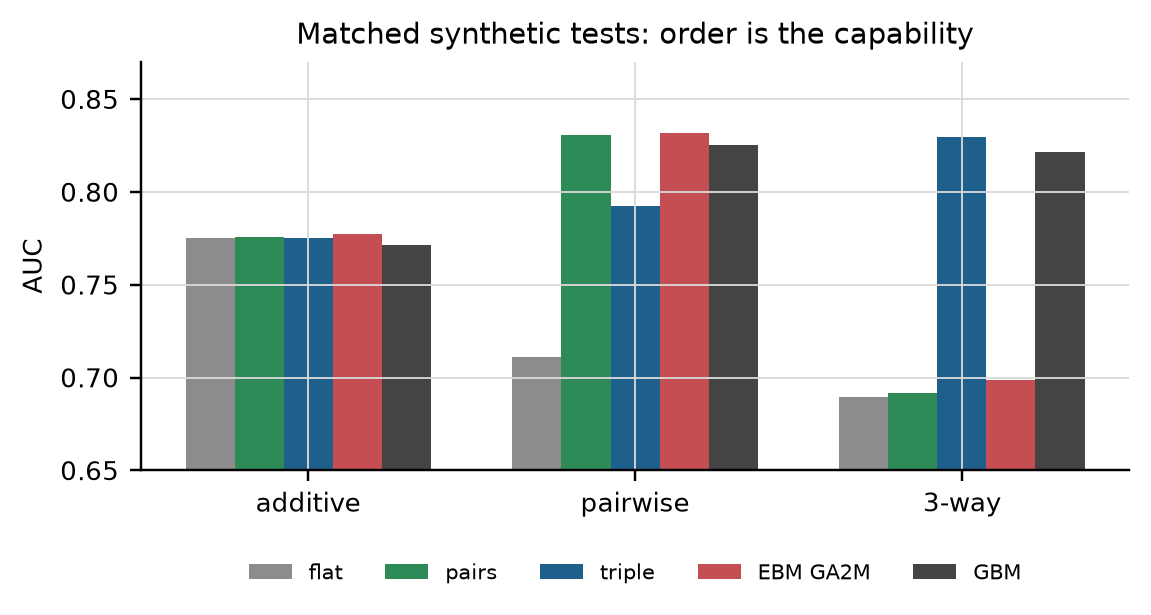
\includegraphics[width=0.78\linewidth]{fig_synthetic}
  \caption{Matched synthetic tests. Each group is a known truth: additive,
  pairwise, or 3-way. Bars are test AUC over three seeds. On the 3-way truth,
  TermGraph (triple) reaches $0.8297$ versus $0.6989$ for pairwise EBM and
  $0.8217$ for the unconstrained GBM. EBM cannot represent the signal by
  construction.}
  \label{fig:synthetic}
\end{figure}


\section{Discussion}

The exact part of TermGraph is the term ledger. Every prediction is a bias plus
a sum of terms, so the ledger adds up by construction. The table compiler is
exact when the source term is constant on the cells of its edges, and the
certified KIRK fold meets that condition to floating-point noise. Feature
values are a different object: they use the declared sharing matrix $W$, and
they are not full-model Shapley when terms overlap. The controller is a budget
selector over expected performance; it does not provide a non-inferiority
guarantee.

EBM remains the stronger low-order model. On KIRK it beats the compact
five-term artifact on raw AUC, and it is the right choice when the effective
order is at most two. TermGraph is useful when the data needs order 3 and when
the artifact must stay editable. This is why the paper reports both the max and
compact artifacts rather than a single winner.

The main structural caveat is identifiability. Overlapping terms are not
unique, so the max artifact's ledger is exact for the declared EBM term set but
is not a canonical functional-ANOVA decomposition. The compact artifact is a
partition, which makes it the cleaner formal object.

The study covers one real task, KIRK, with external data and an external
teacher. I do not include a human user study, categorical or missing-value
benchmarks, multi-class objectives, or training on the full 100k archive. The 3D
term is inspected through slices; cell count alone is not readability.

The runtime is a sum of lookup tables. There are no dense matrix
multiplications and no multiplications, and the terms are independent. The
fused kernel and the binary NPZ artifact are the deployment path evaluated here.

\section{Conclusion}

TermGraph turns a GBM-class model into a certified sum of low-order terms. On
KIRK it matches the EBM plus order-3 hybrid to floating-point noise and reaches
$0.9427$ AUC against $0.9417$ for EBM and $0.9206$ for NAM. A five-term artifact
reaches $0.9296$ at a five-term budget, and the controlled 3-way test gives
$0.8297$ against $0.6989$ for EBM. The same artifact runs at $5.66$M rows/s on
eight threads and ships as a $0.66$~MB NPZ file.

The evidence is limited to KIRK and the controlled benchmark. EBM remains the
better low-order model. Within that boundary, TermGraph carries a GBM into a
table graph with an exact ledger and editable terms, which the fixed-order
glassboxes do not offer.

\section*{Data and code availability}

The code, paper source, figures, and compiled artifacts are available in the
TermGraph repository,
\texttt{github.com/\allowbreak AleeeeM2008/\allowbreak termgraph}. The KIRK
data and the SPOCK teacher are external resources; the repository includes the
derived caches, certificates, and artifacts used in this paper.

\section*{Competing interests}

The author declares no competing interests.

\section*{Disclosure}

This code was assisted by DeepSeek V4.1 Flash to speed up investigation. The
architecture, logic, experiment design, and verification were human-designed and
reviewed; the assistant was used for implementation, plotting, and manuscript
drafting. All reported results are reproducible from the included artifacts and
scripts.

\begin{thebibliography}{99}
\small\raggedright
\bibitem[Chen and Guestrin(2016)]{chen2016xgboost} T. Chen and C. Guestrin. XGBoost: A scalable tree boosting system. KDD, 2016.
\bibitem[Ke et al.(2017)]{ke2017lightgbm} G. Ke et al. LightGBM: A highly efficient gradient boosting decision tree. NeurIPS, 2017.
\bibitem[Prokhorenkova et al.(2018)]{prokhorenkova2018catboost} L. Prokhorenkova et al. CatBoost: Unbiased boosting with categorical features. NeurIPS, 2018.
\bibitem[Lundberg and Lee(2017)]{lundberg2017shap} S. M. Lundberg and S.-I. Lee. A unified approach to interpreting model predictions. NeurIPS, 2017.
\bibitem[Lundberg et al.(2020)]{lundberg2020tree} S. M. Lundberg et al. From local explanations to global understanding with explainable AI for trees. Nature Machine Intelligence, 2020.
\bibitem[Hastie and Tibshirani(1990)]{hastie1990gam} T. Hastie and R. Tibshirani. Generalized Additive Models. Chapman \& Hall, 1990.
\bibitem[Lou et al.(2012)]{lou2012intelligible} Y. Lou, R. Caruana, and J. Gehrke. Intelligible models for classification and regression. KDD, 2012.
\bibitem[Lou et al.(2013)]{lou2013accurate} Y. Lou, R. Caruana, J. Gehrke, and G. Hooker. Accurate intelligible models with pairwise interactions. KDD, 2013.
\bibitem[Agarwal et al.(2021)]{agarwal2021nam} R. Agarwal et al. Neural additive models: Interpretable machine learning with neural nets. NeurIPS, 2021.
\bibitem[Nori et al.(2019)]{nori2019interpretml} H. Nori et al. InterpretML: A unified framework for machine learning interpretability. arXiv:1909.09223, 2019.
\bibitem[Rudin(2019)]{rudin2019stop} C. Rudin. Stop explaining black box machine learning models for high stakes decisions and use interpretable models instead. Nature Machine Intelligence, 2019.
\bibitem[Tamayo et al.(2020)]{tamayo2020spock} D. Tamayo et al. Predicting the stability of planetary systems with deep learning. PNAS, 2020.
\bibitem[Thadhani et al.(2025)]{thadhani2025spock} J. Thadhani, K. Ba, H. Rein, and D. Tamayo. SPOCK 2.0. RNAAS, 2025.
\bibitem[Hussain and Tamayo(2020)]{hussain2020shadows} N. Hussain and D. Tamayo. The effects of chaos on planetary stability. MNRAS, 2020.
\bibitem[Rein and Tamayo(2017)]{rein2017rebound} H. Rein and D. Tamayo. REBOUND: An open-source multi-purpose N-body code. MNRAS, 2017.
\end{thebibliography}

\end{document}
